\documentclass[conference]{IEEEtran}



\usepackage[utf8]{inputenc}

\usepackage{amsmath}

\usepackage{amssymb}

\usepackage{amsfonts}

\usepackage{graphicx}

\usepackage{xurl}

\usepackage{booktabs}

\usepackage{multirow}

\usepackage{cite}

\usepackage{microtype}

\usepackage[hidelinks]{hyperref}

\usepackage{cleveref}



\newcommand{\rltwo}{RL\textsuperscript{2}}



\title{Memory Buys Adaptation, Demonstrations Buy Competence: In-Context Reinforcement Learning Under Real-Time Constraints}



\author{

\IEEEauthorblockN{Felix Surjodinoto}

\IEEEauthorblockA{\textit{Computer Science Department}\\

\textit{School of Computer Science}\\

\textit{Bina Nusantara University}\\

Jakarta 11530, Indonesia\\

\textit{felix.surjodinoto@binus.ac.id}}

\and

\IEEEauthorblockN{Keandre Rafael}

\IEEEauthorblockA{\textit{Computer Science Department}\\

\textit{School of Computer Science}\\

\textit{Bina Nusantara University}\\

Jakarta 11530, Indonesia\\

\textit{keandre.rafael@binus.ac.id}}

\and

\IEEEauthorblockN{Delroy}

\IEEEauthorblockA{\textit{Computer Science Department}\\

\textit{School of Computer Science}\\

\textit{Bina Nusantara University}\\

Jakarta 11530, Indonesia\\

\textit{delroy@binus.ac.id}}

\and

\IEEEauthorblockN{Samuel Philip}

\IEEEauthorblockA{\textit{Computer Science Department}\\

\textit{School of Computer Science}\\

\textit{Bina Nusantara University}\\

Jakarta 11530, Indonesia\\

\textit{samuel.philip@binus.ac.id}}

}



\begin{document}

\raggedbottom



\maketitle



\begin{abstract}

Real-time control denies reinforcement learning its usual luxuries: the simulator neither pauses while the policy computes nor runs faster than the wall clock. We study what it takes to obtain both \emph{competence} and \emph{rapid adaptation} under these constraints, comparing a reactive convolutional agent and causal-transformer \rltwo{} agents on a real-time racing task (20\,Hz, TrackMania 2020) and a controlled blocking benchmark (MuJoCo). On the adaptation side, a transformer \rltwo{} agent trained on action-value faults only transfers its in-context adaptation to an unseen fault \emph{mechanism}: with a no-history ablation isolating adaptation from robustness, the adaptation gap on held-out action latency is $+652 \pm 225$ return (95\% CI, $n{=}3$ seeds, all positive). On the competence side, a demonstration-anchored reactive agent (behavior-cloning warm start from 23 human laps, a pinned demonstration pool in half of every batch, deterministic-episode collection) reaches deterministic track completion within one day of real-time training, whereas transformer agents fall short on identical demonstrations: first under a defective sequence replay, then under six documented failure mechanisms specific to sequence replay and shared trunks, each with its mitigation. Across every run, deterministic-policy failures traced to evaluation states missing from the training distribution: replay design, not architecture, decided the outcome. Memory buys adaptation; demonstrations buy competence.

\end{abstract}



\begin{IEEEkeywords}

Reinforcement learning, real-time control, in-context learning, meta-learning, learning from demonstration, sequence replay.

\end{IEEEkeywords}



\section{Introduction}

\label{sec:introduction}



Deep reinforcement learning has become a standard tool for continuous control, with off-policy actor-critic methods~\cite{ddpg,td3,sac} and high-UTD ensemble variants~\cite{redq,droq,crossq} reaching strong sample efficiency on simulated benchmarks. Transferring this progress to physical vehicles is hard: training on hardware is unsafe and slow, and, more fundamentally, standard RL environments are \emph{blocking}, meaning the simulator pauses while the policy computes, so the learned policy never experiences the execution latency, fixed control intervals, and concurrent time flow of a real control loop~\cite{rtrl,delayedmdp}. TrackMania 2020 offers a useful middle ground: a high-fidelity driving simulator that cannot be paused, imposing real-time constraints identical in kind to a physical vehicle's without the safety cost. We use it as the deployment target of our framework.



Deployed controllers face a further challenge that sample efficiency does not address: \emph{faults}. An actuator degrades, locks, or starts responding with delay, and the controller must compensate online, without gradient updates. In-context meta-RL in the \rltwo{} family~\cite{rl2,wang2016learning,amago} is a natural candidate, since a sequence-model policy can infer the active perturbation from its own action-consequence history. However, existing evaluations test adaptation to unseen \emph{parameters} of training task families; whether in-context adaptation transfers to an unseen fault \emph{mechanism}, a structurally different corruption class, is to our knowledge untested. Moreover, a high return under a held-out fault conflates two explanations: genuine in-context adaptation, or a merely \emph{robust} memoryless policy. Distinguishing them requires an ablation that removes context while changing nothing else.



In-context capability, however, is only half of the question for a deployed system; the other half is whether the machinery that provides it survives real-time training at all. We therefore train three agents on the same racing task: a transformer \rltwo{} agent with a defective sequence replay (whose post-hoc diagnosis motivates the rest), a demonstration-anchored reactive convolutional agent, and a corrected transformer agent trained on identical demonstrations. The reactive agent reaches deterministic track completion within one day of real-time training; the sequence agents do not, and each obstacle they meet is attributable to sequence replay and shared-trunk training rather than to the architecture's representational capacity.



The contributions of this paper are:

\begin{itemize}

    \item \textbf{A controlled fault-adaptation study with a no-history ablation}: training on action-value corruptions only and evaluating on held-out fault splits, the same weights are run with and without context memory. The cross-mechanism adaptation gap (action latency, never trained on) is $+652 \pm 225$ return (95\% CI over 3 seeds, all positive).

    \item \textbf{A demonstration-anchored recipe for real-time competence}: behavior-cloning warm start from 23 human laps ($\approx$30 minutes of demonstrator time), an RLPD-style pinned demonstration pool filling half of every batch~\cite{rlpd}, random-shift image augmentation~\cite{drq}, layer-normalized critics~\cite{droq}, and collection of deterministic-policy episodes into the replay buffer. The resulting reactive agent completes the track deterministically within one day of 20\,Hz real-time training.

    \item \textbf{A deployment-cost study of in-context agents}: six failure mechanisms specific to sequence replay and shared-trunk training, each diagnosed from training telemetry and mitigated (terminal-inclusive variable-length windows, episode-start oversampling, critic-warmup feature freezing, and a behavior-cloning anchor that maintains trunk and encoder features rather than only the policy head).

    \item \textbf{A stabilized transformer \rltwo{} agent}: a causal-transformer context encoder trained by sequence-level REDQ-SAC with layer-normalized critic heads~\cite{droq} and a detached actor head; the real-time configuration additionally supports a Neural ODE block for continuous-time latent modeling~\cite{neuralode} and a RESeL-style context-encoder learning-rate split~\cite{resel}, on a distributed real-time architecture with a 20\,Hz control loop enforced by \texttt{rtgym}~\cite{rtgym,tmrl}.

\end{itemize}



We do not claim a new algorithm: the agents are assembled from established components, and we make no state-of-the-art comparison against systems such as AMAGO~\cite{amago}. The scientific contribution is the mechanism-level transfer question and the ablation that answers it, the demonstration-anchored real-time recipe, and an honest, mechanism-level account of what in-context machinery costs in a deployed real-time system.



\section{Related Work}

\label{sec:related_work}



\subsection{Off-Policy RL and Sample Efficiency}

Off-policy actor-critic methods~\cite{ddpg,td3} and maximum-entropy SAC~\cite{sac} dominate continuous control. Raising the update-to-data (UTD) ratio improves sample efficiency but destabilizes value learning. REDQ~\cite{redq} maintains an ensemble of $N$ critics and computes Bellman targets from the minimum over a random subset of size $M$; DroQ~\cite{droq} achieves similar control with dropout and layer normalization inside the critics; CrossQ~\cite{crossq} removes target networks via batch normalization. Distributed actor-learner systems~\cite{apex} decouple collection from optimization, which our architecture adopts in a real-time setting.



\subsection{Real-Time RL and Delayed MDPs}

Real-time RL~\cite{rtrl} formalizes the setting where the environment advances while the agent computes; delayed-MDP theory~\cite{delayedmdp} and random-delay methods~\cite{bouteiller2021delays} treat action/observation latency explicitly. Real-Time Gym (\texttt{rtgym})~\cite{rtgym} enforces fixed control intervals: observations are captured at interval boundaries, actions are applied exactly one interval later, and computation overruns are handled elastically instead of pausing the simulator. Our control loop builds directly on it, and action latency reappears in our benchmark as the held-out cross-mechanism fault.



\subsection{In-Context Meta-RL, Fault Adaptation, and Neural ODEs}

\rltwo{}~\cite{rl2,wang2016learning} trains recurrent policies that implement a learned RL procedure in their hidden-state dynamics; PEARL~\cite{pearl} infers an explicit probabilistic task variable off-policy; Decision Transformer~\cite{decisiontransformer} and AMAGO~\cite{amago} replace the RNN with transformers. All evaluate held-out \emph{parameters} of training task families. For fault recovery specifically, GrBAL~\cite{grbal} and FAMLE~\cite{famle} meta-learn dynamics models that adapt online to perturbed dynamics drawn from the training family, and domain randomization~\cite{tobin2017domain} trains policies robust to wide distributions, which is exactly the explanation our no-history ablation isolates. Neural ODEs~\cite{neuralode} model hidden states as continuous-time dynamical systems $\mathrm{d}h/\mathrm{d}\tau = f(h)$, a natural fit for latents that must remain consistent under continuous time flow and actuation latency.



\subsection{Learning from Demonstrations}

Demonstrations address precisely the resource that real-time RL lacks: exploration paid in wall-clock time. DQfD~\cite{dqfd} pretrains on demonstrations and keeps them in replay with an imitation margin loss; RLPD~\cite{rlpd} shows that simply composing half of every batch from a pinned offline buffer, together with layer-normalized critics and high update ratios, matches more elaborate offline-to-online methods; random-shift augmentation~\cite{drq} is the standard regularizer for pixel-based actor-critic learning. Our reactive deployment recipe combines these three with a behavior-cloning warm start, and our sequence agent extends the anchor idea: when the actor head reads a shared trunk through a stop-gradient, an imitation loss confined to the head cannot prevent the critic from repurposing the features beneath it, so the anchor must backpropagate into the encoder.



\subsection{Recurrent and Transformer Stability in Off-Policy RL}

Sequence replay has its own failure modes, first catalogued for recurrent value functions by R2D2~\cite{r2d2}: stored-state staleness, burn-in, and the mismatch between the state distributions of training windows and deployment. Our deployment study adds image-scale variants of this catalogue, including a starvation effect in which uniform window sampling almost never trains the short-context episode-start states the deployed policy must handle after every reset. When critics share a recurrent or transformer trunk, high-UTD critic gradients additionally dominate the shared representation, causing oversaturation and catastrophic forgetting. RESeL~\cite{resel} shows that recurrent off-policy RL requires a context-encoder-specific (lower) learning rate. We adopt this two-group optimization in the real-time deployment configuration, and in the controlled benchmark we report direct evidence (\cref{sec:stability}) that layer-normalized critic heads were necessary in our setting, where ensemble critics sharing one trunk are highly correlated and min-based pessimism is weakened.



\section{System Architecture and Methodology}

\label{sec:methodology}



\subsection{Distributed Architecture and Real-Time Control Loop}

TMRL adopts a decoupled client-server architecture: rollout workers co-located with the TrackMania 2020 simulator execute the current policy and buffer transitions; a central broker relays data and weights over the \texttt{tlspyo} library~\cite{tlspyo}; a GPU trainer aggregates experience, performs the gradient updates, and periodically broadcasts new weights. The control loop is enforced by Real-Time Gym (\texttt{rtgym})~\cite{rtgym} at a fixed 20\,Hz ($\Delta t = 0.05$\,s): the observation is captured at the interval's start boundary, the action is applied via a virtual gamepad exactly at the end boundary, and computation overruns are handled elastically instead of pausing the simulator.



\subsection{Action and Observation Spaces}

The action is $a_t = [g_t, b_t, s_t] \in [-1, 1]^3$ (gas, brake, steering). Observations are grayscale screenshots resized to $64 \times 64$ (the reactive agent stacks 4 frames; the sequence agents use a single frame per step, the transformer history supplying temporal context), telemetry (speed, gear, engine RPM) retrieved via the OpenPlanet API~\cite{openplanet}, and the previously applied actions.



\subsection{Transformer \rltwo{} Trunk and Task-Inference Head}

\label{sec:trunk}

For in-context adaptation, each timestep is embedded as one token: a linear \emph{timestep embedder} projects $[\,s_t \,\|\, a_{t-1} \,\|\, r_{t-1} \,\|\, d_{t-1}\,]$ to $d_{\text{model}} = 64$, where $d$ is an episode-boundary indicator; in the visual configuration a per-timestep CNN first encodes the image stack to a 128-dimensional feature. The token sequence, plus learned positional embeddings, passes through a 2-layer pre-norm causal transformer (2 heads, feed-forward width 128, dropout 0.1, GELU, context window up to 128 tokens), yielding per-token hidden states $h_t \in \mathbb{R}^{64}$. At inference the actor keeps a deque of recent timesteps and re-runs the forward pass each step (negligible cost at this scale); the deque is cleared on episode boundaries, so context never leaks across episodes.



A small \emph{task encoder} maps each $h_t$ to an 8-dimensional task embedding $z_t$, which conditions both actor and critic heads, and to classification logits over the fault taxonomy, trained with an auxiliary cross-entropy loss against the episode's ground-truth fault label (training-time only; weight $\lambda_{\text{task}} = 0.05$). This gives the trunk an explicit incentive to encode fault identity rather than relying solely on the return objective.



\subsection{Continuous-Time Latent Dynamics via Neural ODEs}

\label{sec:node}

The output hidden state of the causal transformer trunk is modeled as a continuous-time dynamical system:

\begin{equation}

    \frac{dh(\tau)}{d\tau} = f(h(\tau), \theta_{\text{ODE}})

\end{equation}

where $f$ is a multi-layer perceptron consisting of Layer Normalization, a linear layer, GELU activation, and a final linear layer. To stabilize the start of training, the final layer's weights are initialized to zero, making $f(h, \theta_{\text{ODE}}) \approx 0$ initially, so the block begins as the identity.



We integrate the latent state over a virtual duration $\Delta\tau$ (\texttt{ode\_dt} = 1.0) using $K$ fixed steps $\delta\tau = \Delta\tau / K$ with either the explicit Euler scheme, $h_{k+1} = h_k + \delta\tau \, f(h_k, \theta_{\text{ODE}})$, or the classical fourth-order Runge--Kutta scheme; the final integrated state $h_K$ is passed to the policy and critic heads. This block targets the latency-afflicted real-time setting; the controlled benchmark experiments of \cref{sec:experiments} disable it, keeping the headline result attributable to the context mechanism alone.



\subsection{Stabilized Off-Policy Sequence Training}

\label{sec:training}

The learning algorithm is a sequence-level adaptation of REDQ-SAC~\cite{redq,sac}: an ensemble of $N = 10$ critic heads shares the transformer trunk, and Bellman targets use the minimum over a random subset of $M = 2$ target critics with entropy-regularized SAC targets and a learned temperature. Replay stores whole trajectories; each gradient step samples windows of $L_{\text{burn}} + L_{\text{train}}$ consecutive timesteps ($8 + 24$ in the controlled benchmark, $20 + 64$ in the TrackMania configuration), where the first $L_{\text{burn}}$ positions condition the trunk but are masked out of all losses. The episode-boundary flag is terminated-only (truncation does not set it), consistent with the terminated-only bootstrap in the sequence memory. Throughout this paper, UTD denotes the number of critic updates per policy update (the implementation's \texttt{q\_updates\_per\_policy\_update}), not gradient steps per environment step.



At high UTD the shared trunk receives many more critic gradients than actor gradients, leading to representation oversaturation and catastrophic forgetting as the buffer saturates. Two measures protect the trunk in all configurations: the actor head reads trunk features through a stop-gradient (at UTD 10--15 critic gradients outnumber actor gradients by an order of magnitude), and each critic head is a 2-hidden-layer MLP with LayerNorm after every hidden linear layer~\cite{droq}, which proved essential in practice (\cref{sec:stability}). The real-time configuration additionally follows RESeL~\cite{resel}, dividing parameters into two optimization groups, the context encoder (transformer trunk, embedder, and Neural ODE) and the task heads (policy and critics), with a reduced context learning rate

\begin{equation}

    \eta_{\text{context}} = \gamma_{\text{RESeL}} \cdot \eta_{\text{heads}},

\end{equation}

where $\gamma_{\text{RESeL}} = 0.1$ by default and $\eta_{\text{context}}$ may instead be set explicitly (our deployment run uses $\eta_{\text{context}} = 5 \times 10^{-5}$). The controlled benchmark runs do not enable this split: there, the context encoder trains at the full critic learning rate, so the benchmark results isolate the contribution of the context mechanism without RESeL.



\subsection{Demonstration-Anchored Real-Time Training}

\label{sec:demos}

Because the simulator runs strictly in real time, exploration is bounded by the wall clock: at 20\,Hz, a day of training yields at most $1.7 \times 10^6$ transitions regardless of compute. We therefore anchor deployment training on human demonstrations, recorded by replacing the policy with a reader of the demonstrator's input device while routing observations, rewards, and resets through the unmodified pipeline (so recorded transitions are distributionally identical to agent experience; unfinished episodes are rejected). Twenty-three complete laps (26{,}642 transitions, $\approx$30 minutes of demonstrator time, best lap $\approx$54\,s) anchor training three ways: a behavior-cloning warm start; an RLPD-style pinned demonstration pool~\cite{rlpd} filling half of every batch and never evicted (which doubles as an anti-forgetting mechanism); and, for the sequence agent, a behavior-cloning anchor term in the actor loss. Additionally, every $k$-th training episode is collected \emph{with the deterministic policy} and sent to replay, so deterministic failure modes become training data, and random-shift augmentation~\cite{drq} regularizes the image pathway.



\subsection{Terminal-Aware Sequence Replay}

\label{sec:seqreplay}

The deployment study (\cref{sec:tm_exp}) traces most sequence-agent failures to the replay. The corrected design differs from a naive window sampler in four ways. \emph{Terminal inclusion}: variable-length windows run up to and including the episode's final step, so terminal rewards enter training; termination zeroes the bootstrap while truncation bootstraps from the real successor. \emph{Short-episode support}: episodes shorter than the window are right-padded and masked instead of discarded. \emph{Episode-start oversampling}: uniform offset sampling yields one episode-start window per $\sim$1{,}130 mid-episode windows, starving the short-context launch behavior required after every reset (and starving behavior-cloning pretraining, which uses the same sampler); a fixed fraction (0.25) of windows is forced to begin at episode starts. \emph{Feature-maintaining anchor}: the behavior-cloning anchor backpropagates through non-detached hidden states into the encoder at the slow context rate, while the value term still reaches only the head; without this, the critic, which alone trains the shared trunk and CNN, continuously repurposes the features under the actor head.



\subsection{Fault-Injection Benchmark and the No-History Ablation}

\label{sec:benchmark}

To evaluate in-context adaptation under control, a wrapper turns any flat-\texttt{Box} Gymnasium~\cite{gymnasium} environment into an \rltwo{} task: it packs $(a_{\text{prev}}, r_{\text{prev}}, d_{\text{prev}})$ into the observation tuple and draws one unobservable fault per episode from the taxonomy in \cref{tab:faults}. The stored $a_{\text{prev}}$ is the \emph{commanded} (pre-fault) action, so the agent observes what it asked for and then the corrupted consequence; that discrepancy is the meta-learning signal. Formally, the agent commands $a_t$ and the environment executes $\tilde{a}_t = g_\phi(a_t, h_t)$ for episode fault $\phi$, with $\operatorname{supp}(p_{\text{eval}}) \cap \operatorname{supp}(p_{\text{train}}) = \emptyset$ at test time, and the policy is the sequence model $a_t \sim \pi_\theta(\cdot \mid s_{\leq t}, a_{<t}, r_{<t}, d_{<t})$.



\begin{table}[!t]

\centering

\caption{Fault taxonomy. Severity $s \in [0,1]$; experiments use $s=1$. Faults are resampled each episode and are not observable.}

\label{tab:faults}

\begin{tabular}{llp{3.5cm}}

\toprule

\textbf{Fault} & \textbf{Mechanism} & \textbf{Effect (per episode)} \\

\midrule

\texttt{action\_scale}   & value     & each action dim.\ scaled by $u \sim \mathcal{U}[1{-}0.5s,\, 1{+}0.5s]$ \\

\texttt{action\_noise}   & value     & i.i.d.\ Gaussian noise, std.\ $0.5s$, added to actions \\

\texttt{sensor\_noise}   & value (obs.) & i.i.d.\ Gaussian noise, std.\ $0.5s$, added to observations \\

\texttt{dead\_actuator}  & value (extreme) & one random action dim.\ locked to $0$ \\

\texttt{sign\_flip}      & value (extreme) & one random action dim.\ negated \\

\texttt{action\_latency} & \textbf{temporal} & executed action is the one commanded $k$ steps ago, $k \sim \mathcal{U}\{1,\dots,5\}$ \\

\bottomrule

\end{tabular}

\end{table}



Training draws uniformly from the value-corruption faults \texttt{action\_scale} and \texttt{action\_noise}. Evaluation uses two disjoint held-out splits: \textbf{within-mechanism extrapolation} (\texttt{dead\_actuator}, \texttt{sign\_flip}: still per-dimension value corruption, but at gains of $0$ and $-1$ when training never goes below $0.5$) and \textbf{cross-mechanism} transfer (\texttt{action\_latency}: action values preserved but delayed by $k$ steps, a temporal corruption absent from training).



To attribute held-out performance correctly, every evaluation runs the identical weights twice: \textbf{adaptive} (the context deque accumulates the episode history) and \textbf{no-history} (the deque is cleared before every action selection, reducing the agent to a nearly memoryless reactive policy). The \emph{adaptation gap} $G = R_{\text{adaptive}} - R_{\text{no-history}}$ measures exactly the contribution of in-context memory: a robust history-independent policy gives $G \approx 0$, whereas genuine in-context adaptation gives $G > 0$. The ablation costs one extra evaluation pass and no retraining.



\section{Experimental Evaluation}

\label{sec:experiments}



\subsection{Controlled Fault-Adaptation Experiments}

\label{sec:fault_exp}

The base environment is HalfCheetah-v5 (MuJoCo~\cite{mujoco}; 17-dimensional observations, 6 actuators), with the Neural ODE block and the RESeL split disabled. Agents train for up to $10^3$ iterations of \{4 collection episodes $\rightarrow$ 100 gradient steps\} at UTD 10 (critic updates per policy update), batch 64, replay $10^6$, Adam (actor $3{\times}10^{-4}$; critic and context encoder $1.5{\times}10^{-4}$; entropy $3{\times}10^{-4}$), $\gamma = 0.99$, polyak 0.995, gradient clip 10, on the train-fault distribution only. Every 25 iterations the agent is evaluated on the held-out faults and the best held-out checkpoint per seed is retained. Final numbers evaluate each seed's best checkpoint for 25 deterministic episodes per condition, with and without history, over $n = 3$ seeds; we report mean $\pm$ 95\% CI of the per-seed gaps. The two configurations differ only in the held-out evaluation set.



\begin{table}[!t]

\centering

\caption{Mean return of the best checkpoint per seed under held-out faults, adaptive vs.\ no-history. Gap is mean $\pm$ 95\% CI over $n{=}3$ seeds.}

\label{tab:results}

\begin{tabular}{lccc}

\toprule

\textbf{Held-out condition} & \textbf{Adaptive} & \textbf{No-history} & \textbf{Gap} \\

\midrule

Cross-mechanism & \multirow{2}{*}{$+312.7$} & \multirow{2}{*}{$-339.6$} & $\mathbf{+652.3 \pm 224.7}$ \\

(\texttt{action\_latency}) & & & (CI excludes 0) \\

\addlinespace

Within-mechanism & \multirow{2}{*}{$+344.8$} & \multirow{2}{*}{$-356.7$} & $+701.4 \pm 770.6$ \\

(\texttt{dead}/\texttt{sign\_flip}) & & & (CI includes 0) \\

\bottomrule

\end{tabular}

\end{table}



\begin{figure*}[!t]

    \centering

    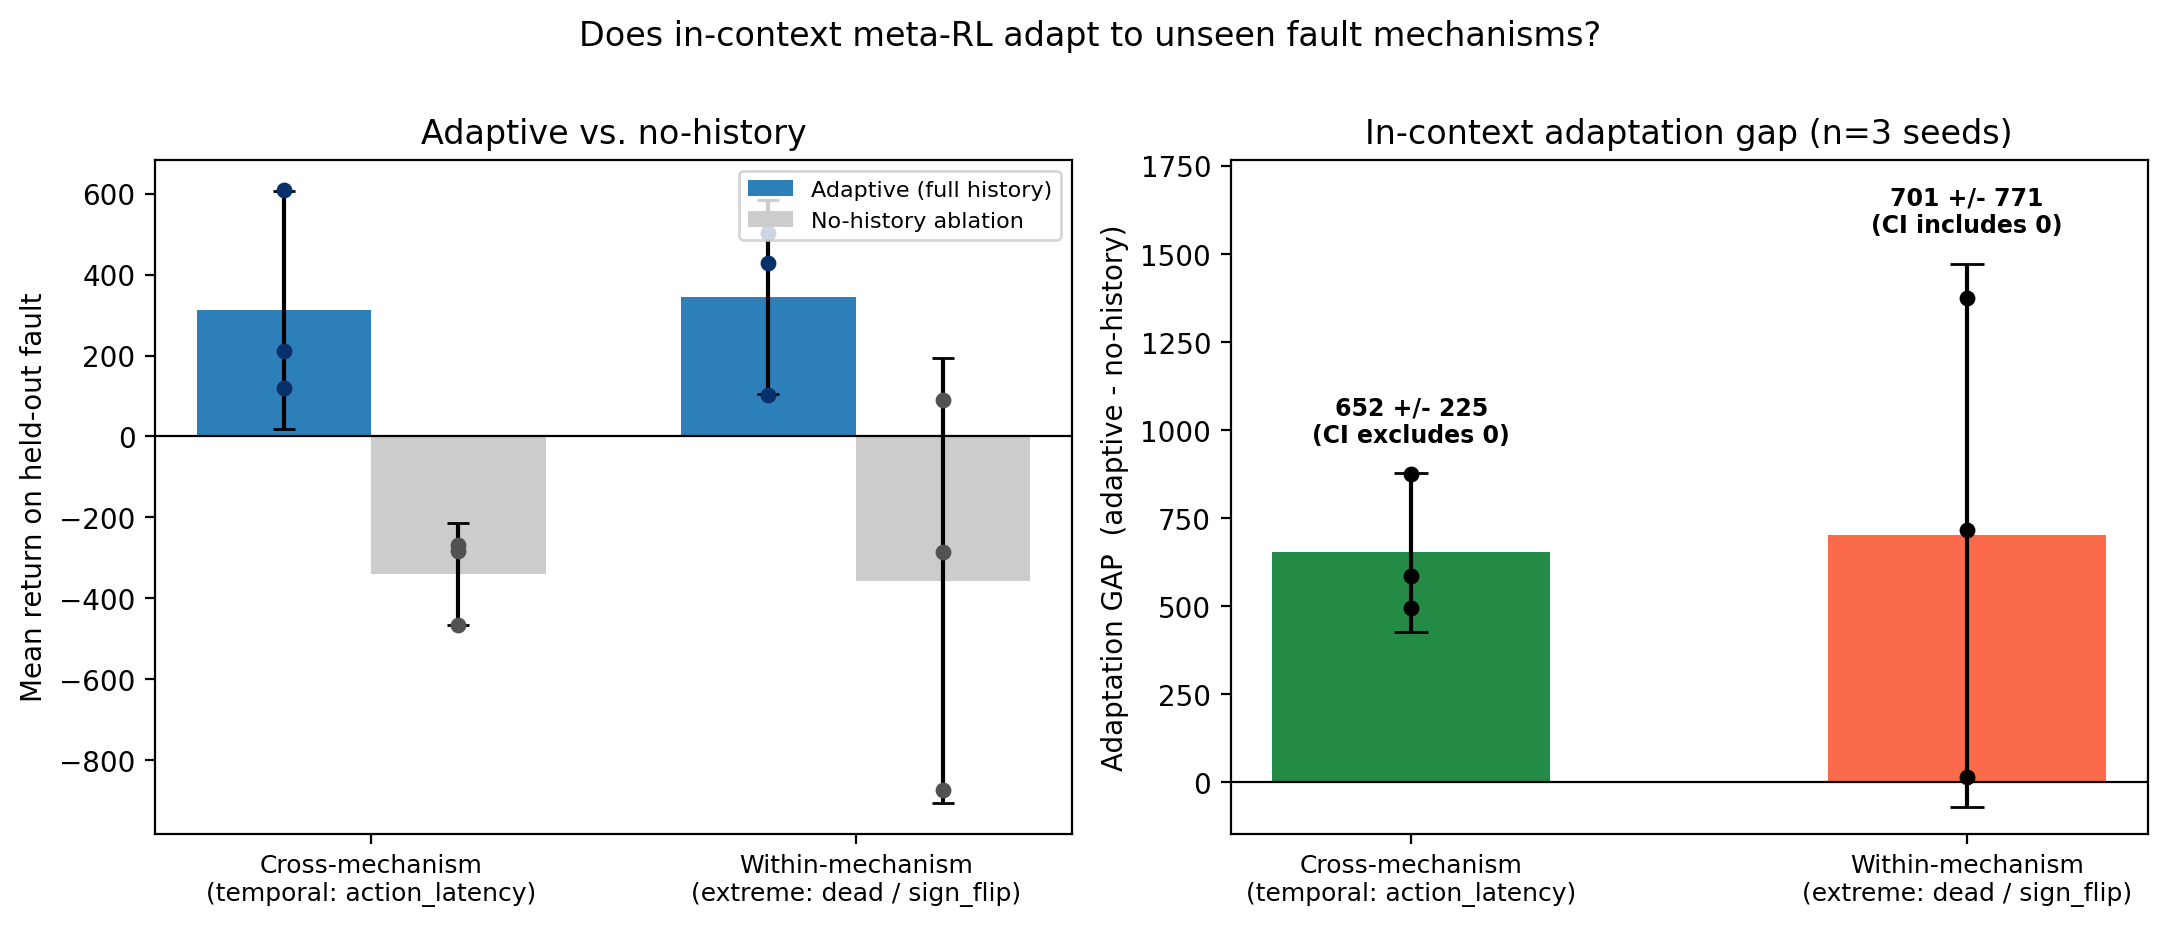
\includegraphics[width=0.92\textwidth]{fault_adaptation_result.png}

    \caption{In-context adaptation on held-out fault classes (HalfCheetah, 3 seeds, best checkpoint per seed, 25 deterministic episodes per condition). \textbf{Left:} mean return of the same trained weights evaluated with full history (blue) and with memory reset every step (gray); dots are individual seeds. \textbf{Right:} the per-condition adaptation gap with 95\% CIs. The cross-mechanism gap ($+652 \pm 225$) excludes zero with all three seeds positive; the within-mechanism gap is larger on average but seed-dependent.}

    \label{fig:fault_adaptation}

\end{figure*}



\Cref{tab:results} and \cref{fig:fault_adaptation} present the result. On \texttt{action\_latency}, a fault mechanism with zero overlap with training, the adaptive policy averages $+312.7$ return while its memoryless self averages $-339.6$, an adaptation gap of $+652.3 \pm 224.7$ whose confidence interval excludes zero; the per-seed gaps are $+495$, $+586$, and $+876$, positive on every seed. The agent is not merely robust to delay; it uses within-episode evidence to behave differently, and much better, than the same weights without memory. The in-context inference machinery learned on value-corruption faults generalizes to a temporally structured fault it has never encountered.



On dead/sign-flipped actuators the mean gap is larger ($+701.4$) but the per-seed gaps are $+715$, $+1376$, and $+14$: one seed gains essentially nothing, inflating the CI to $\pm 770.6$. We report this as suggestive rather than established. The asymmetry is notable: extreme extrapolation within the trained mechanism appears harder to exploit reliably than transfer to a structurally different but dynamically milder fault. In both conditions the no-history evaluation is strongly negative, as expected for a policy trained exclusively as a history-conditioned model; the gap therefore reads as ``how much work the context is doing,'' not as a comparison against a tuned robust baseline, which remains future work.



\subsubsection{Stability Finding: LayerNorm Critic Heads}

\label{sec:stability}

With plain MLP critic heads, training under this exact configuration ($M{=}2$, critic LR $1.5{\times}10^{-4}$, UTD 10) entered value divergence: Q-estimates climbed toward ${\sim}50$ and the critic loss toward ${\sim}150$, after which the policy collapsed. A single-variable change, enabling LayerNorm in the critic heads, eliminated the divergence in our runs while preserving peak held-out performance. REDQ's min-over-$M$ pessimism is weakened when all ensemble members share one transformer trunk (their errors are correlated); bounding head activations restores the missing regularization, consistent with DroQ~\cite{droq}.



\subsection{Real-Time Evaluation on TrackMania 2020}

\label{sec:tm_exp}

We trained three agents on the same track under the visual configuration ($64{\times}64$ grayscale screenshots, OpenPlanet telemetry, previously applied actions), all three system processes running on one machine over the loopback interface. The track's progress-based reward yields $\approx$180 over a full lap plus a $+100$ completion bonus, so a deterministic return near 280 certifies a completed lap; episodes in which the car fails to progress are terminated by a failure countdown at a floor of 86 steps (return $\approx$5). The demonstrator's best lap is $\approx$54\,s.



\subsubsection{Run A: Transformer \rltwo{} with Defective Sequence Replay}

\label{sec:runa}

The first deployment used the full architecture of \cref{sec:trunk,sec:node,sec:training} (single frame per step, transformer context, Neural ODE, RESeL split, sequence window $20+64$, REDQ-SAC with $N{=}10$, $M{=}2$) with a naive sequence replay and no demonstrations. Training ran in two stages: a high sample-efficiency configuration (UTD 15, target entropy $-1.5$), then an exploration-stabilized resumption (UTD 5, target entropy $-2.5$) responding to the policy drift analyzed below.



\begin{table}[!t]

\centering

\caption{Quantitative progress metrics across training steps (TrackMania 2020, visual configuration, single run).}

\label{tab:epoch_progress}

\resizebox{\columnwidth}{!}{%

\begin{tabular}{ccccccc}

\toprule

\textbf{Phase} & \textbf{Steps} & \textbf{Max Buffer} & \textbf{Mean } $\alpha$ & \textbf{Mean Q} & \textbf{Max Train} & \textbf{Max Test} \\

 & & (\texttt{memory\_len}) & & ($Q_{\theta}$) & \textbf{Return} & \textbf{Return} \\

\midrule

Early    & 0--100   & 153k & 0.0403 & 2.22 & 29.18  & 14.08 \\

Mid-Low  & 101--200 & 338k & 0.0266 & 3.92 & 74.39  & 6.52  \\

Mid      & 201--400 & 697k & 0.0155 & 4.13 & 82.75  & 82.60 \\

High     & 401--600 & 961k & 0.0080 & 4.22 & 116.39 & 105.19 \\

Peak     & 601--750 & 965k & 0.0047 & 4.25 & 97.58  & \textbf{122.49} \\

Drift    & 751--779 & 965k & 0.0038 & 4.23 & 70.16  & 86.77 \\

\midrule

Recovery & 780+     & 965k & 0.0035 & 4.26 & 15.67  & \textbf{86.27} \\

\bottomrule

\end{tabular}%

}

\end{table}



\Cref{tab:epoch_progress} shows the run's progression: the entropy coefficient decayed smoothly, mean Q stabilized near 4.25, and the agent reached a peak deterministic test return of 122.49, well below the completion threshold, before a drift episode following replay-buffer saturation collapsed the test return to 13.92; lowering UTD to 5 and relaxing target entropy recovered 86.27. At the time, we attributed the plateau and drift to high-UTD instability alone.



A post-hoc audit of the replay explains the ceiling more simply. The window sampler only admitted windows containing no episode boundary, so (i) terminal transitions, including the $+100$ completion bonus and all crash endings, never entered training and every sampled target bootstrapped as if episodes were infinite; (ii) episodes shorter than the 85-step window contributed no training data at all, biasing the distribution toward rare long episodes; and (iii) positional embeddings beyond index 84 were never trained although deployed episodes exceeded that length. Under these defects the critic could not represent the value of finishing, and no amount of architectural stabilization could have produced competence. Run A therefore serves as a case study rather than a baseline: its architecture is exonerated, its replay is not.



\subsubsection{Run B: Demonstration-Anchored Reactive Agent}

\label{sec:runb}

The reactive agent replaces the transformer with a feedforward CNN over a 4-frame stack (SAC, two layer-normalized critics), trained with the full demonstration recipe of \cref{sec:demos}: behavior-cloning warm start (held-out validation loss 0.034), the pinned demonstration pool at fraction 0.5, random-shift augmentation, deterministic-episode collection every 4th episode, and target entropy $-6$ (the bang-bang keyboard demonstrations saturate the policy mean, and a conventional target entropy steadily de-saturates it). The behavior-cloned policy alone completed one slow lap (73.6\,s) in three evaluation episodes before any reinforcement learning.



Early training exposed the one blind spot of this recipe: deterministic test episodes collapsed to the 86-step floor while stochastic training episodes kept improving. Test episodes are never collected, so the buffer contained no deterministic-policy failures and the critic could not correct them. Collecting every 4th training episode deterministically made the failure mode training data; deterministic test returns recovered within hours, reaching 168.4 and then \textbf{279.7 at 1{,}372 steps ($\approx$68.6\,s): a deterministic track completion}, with subsequent training episodes finishing consistently (returns 273--280). Total wall-clock from first demonstration to deterministic completion was approximately one day, with the lap $\approx$27\% slower than the demonstrator's best and still improving when the run was stopped.



\subsubsection{Run C: Corrected Sequence Agent on Identical Demonstrations}

\label{sec:runc}

The corrected transformer agent uses the terminal-aware replay of \cref{sec:seqreplay} and the same demonstrations, with behavior cloning applied to the full perception--context--policy path (final loss 0.005). Reaching a stable configuration required diagnosing, in sequence, six failure mechanisms absent from Run B by construction:

\begin{enumerate}

    \item \emph{Sequence batch memory}: 85 timesteps of images per sample oversubscribed an 8\,GB GPU at batch 128 in fp32; bf16 autocast and batch 32--64 reduced training tensors to $<$1\,GB.

    \item \emph{Warmup entropy divergence}: freezing actor and temperature while critics calibrated left the target's entropy term unregulated; the near-deterministic policy's large positive log-likelihoods drove Q-targets toward a negative fixed point within hundreds of steps. Fix: pure policy evaluation during warmup.

    \item \emph{Feature drift under a frozen head}: with the actor head frozen, deployed episode length still degraded from 305 to 86 steps within $\sim$400 critic updates; the critic was rewriting the CNN and trunk under the constant head. A frozen head over a critic-trained trunk is not a frozen policy.

    \item \emph{Episode-start starvation}: uniform window sampling trained launch behavior in $\sim$0.1\% of windows; cloned rollouts launched inconsistently and RL progressively lost the launch. Fix: episode-start oversampling (\cref{sec:seqreplay}).

    \item \emph{Head-only anchoring is insufficient}: anchored at the detached head, the imitation loss equilibrated at 0.10 (weight 5) and 0.073 (weight 15) against 0.005 after pretraining. Routing the anchor gradient into the encoder restored 0.03.

    \item \emph{Exposure bias}: the policy conditions on its own action history, teacher-forced during cloning; deviations compound at deployment. Mitigated, not eliminated.

\end{enumerate}

At the time of writing, the corrected agent trains stably, launches reliably, and sustains deterministic episodes of 140--400 steps, but has not completed the track (\cref{tab:deployment}). We report this asymmetry as a finding: under real-time constraints, the in-context machinery that produces the adaptation gap of \cref{tab:results} carries a systems cost a reactive policy never pays, and on a fixed task that cost so far exceeds its benefit.



\begin{table}[!t]

\centering

\caption{Real-time deployment summary (same track; Runs B and C share identical demonstrations). Completion requires deterministic return $\approx$280.}

\label{tab:deployment}

\resizebox{\columnwidth}{!}{%

\begin{tabular}{lccc}

\toprule

 & \textbf{Run A} & \textbf{Run B} & \textbf{Run C} \\

\midrule

Policy & transformer \rltwo{} & reactive CNN & transformer \rltwo{} \\

Sequence replay & defective & none & corrected \\

Demonstrations & none & 23 laps & 23 laps \\

Peak determ.\ return & 122.5 & \textbf{279.7} & 86.1 \\

Track completion & no & \textbf{yes} ($\approx$68.6\,s) & no \\

\bottomrule

\end{tabular}%

}

\end{table}



This mirrors the high-UTD instability literature~\cite{redq,droq} in a deployed asynchronous setting and motivated the stability measures of \cref{sec:training}. Across all three runs, every deterministic-policy failure (Run A's untrained terminals, Run B's blind spot, Run C's launch starvation) is one principle violated three ways: \emph{the deployed policy visited states that the training distribution did not contain}. Replay design, not architecture, decided each outcome.



\subsection{Limitations}

\label{sec:limitations}

(i) The controlled study uses one MuJoCo task; the harness supports CARL and Meta-World, but those results do not exist yet. (ii) Training is not stable on all seeds; we report best-checkpoint performance, which is standard but optimistic, and the LayerNorm fix removed value divergence, not all instability. (iii) $n{=}3$ seeds is the minimum for a CI, and the within-mechanism result is unresolved at this sample size. (iv) We compare the agent against its own memoryless self, the right comparison for attribution, but not against AMAGO, PEARL, or a domain-randomized policy, so no state-of-the-art claim is made. (v) Absolute returns under faults are modest ($+313$ to $+345$); the claim concerns the source of resilience, not its sufficiency. (vi) The deployment study is one run per configuration on one track, with interventions decided sequentially from training telemetry rather than pre-registered; the Run~B vs.\ Run~C comparison controls demonstrations, track, reward, and learning signal, but not seed variance. (vii) Run~C was still training at the time of writing; its reported status is a lower bound, not a final outcome. (viii) The Neural ODE block and the RESeL split are enabled only in deployment runs and are not individually ablated anywhere; we make no claims about their contribution.



\section{Conclusion and Future Work}

\label{sec:conclusion}

Replay design, not architecture, decided every outcome in this paper. A controlled fault-injection study with a no-history ablation showed that in-context adaptation transfers to an unseen fault \emph{mechanism}: on held-out action latency the adaptation gap is $+652 \pm 225$ return (95\% CI over 3 seeds, all positive). Memory demonstrably buys within-episode adaptation. Under real-time constraints, however, competence came from a different source: a demonstration-anchored reactive agent (behavior-cloning warm start, a pinned demonstration pool in half of every batch, deterministic-episode collection) reached deterministic track completion within one day, while transformer \rltwo{} agents on identical demonstrations did not: first under a defective sequence replay whose post-hoc diagnosis exonerates the architecture, then, in corrected form, under six documented failure mechanisms specific to sequence replay and shared-trunk training. All three deployments failed deterministically wherever the training distribution lacked the states the deployed policy visited: untrained terminals, an uncollected deterministic failure mode, starved episode starts. Memory buys adaptation; demonstrations buy competence; replay design decides whether either is delivered.



Future work: per-component ablations of the deployment stabilizers (Neural ODE, RESeL, task conditioning) on the controlled benchmark, where they currently have no isolated evidence; AMAGO and domain-randomization baselines, more tasks and seeds; completing the corrected sequence agent's run and, if it reaches competence, injecting the fault taxonomy into the racing setting to test whether the adaptation gap survives deployment; and sim-to-real transfer of the demonstration-anchored recipe.



\begingroup

\hbadness=10000

\begin{thebibliography}{99}



\bibitem{ddpg}

T.~P. Lillicrap, J.~J. Hunt, A.~Pritzel, N.~Heess, T.~Erez, Y.~Tassa, D.~Silver, and D.~Wierstra, ``Continuous control with deep reinforcement learning,'' in \emph{International Conference on Learning Representations (ICLR)}, 2016.



\bibitem{td3}

S.~Fujimoto, H.~van Hoof, and D.~Meger, ``Addressing function approximation error in actor-critic methods,'' in \emph{International Conference on Machine Learning (ICML)}, 2018.



\bibitem{sac}

T.~Haarnoja, A.~Zhou, P.~Abbeel, and S.~Levine, ``Soft Actor-Critic: Off-policy maximum entropy deep reinforcement learning with a stochastic actor,'' in \emph{International Conference on Machine Learning (ICML)}, 2018.



\bibitem{redq}

X.~Chen, C.~Wang, Z.~Zhou, and K.~W. Ross, ``Randomized ensembled double Q-learning: Learning fast without a model,'' in \emph{International Conference on Learning Representations (ICLR)}, 2021.



\bibitem{droq}

T.~Hiraoka, T.~Imagawa, T.~Hashimoto, T.~Onishi, and Y.~Tsuruoka, ``Dropout Q-functions for doubly efficient reinforcement learning,'' in \emph{International Conference on Learning Representations (ICLR)}, 2022.



\bibitem{crossq}

A.~Bhatt, D.~Palenicek, B.~Belousov, M.~Argus, A.~Amiranashvili, T.~Brox, and J.~Peters, ``CrossQ: Batch normalization in deep reinforcement learning for greater sample efficiency and simplicity,'' in \emph{International Conference on Learning Representations (ICLR)}, 2024.



\bibitem{rtrl}

S.~Ramstedt and C.~Pal, ``Real-time reinforcement learning,'' in \emph{Advances in Neural Information Processing Systems (NeurIPS)}, 2019.



\bibitem{delayedmdp}

K.~V. Katsikopoulos and S.~E. Engelbrecht, ``Markov decision processes with delays and asynchronous cost collection,'' \emph{IEEE Transactions on Automatic Control}, vol.~48, no.~4, pp. 568--574, 2003.



\bibitem{rl2}

Y.~Duan, J.~Schulman, X.~Chen, P.~L. Bartlett, I.~Sutskever, and P.~Abbeel, ``RL$^2$: Fast reinforcement learning via slow reinforcement learning,'' \emph{arXiv preprint arXiv:1611.02779}, 2016.



\bibitem{wang2016learning}

J.~X. Wang, Z.~Kurth-Nelson, D.~Tirumala, H.~Soyer, J.~Z. Leibo, R.~Munos, C.~Blundell, D.~Kumaran, and M.~Botvinick, ``Learning to reinforcement learn,'' \emph{arXiv preprint arXiv:1611.05763}, 2016.



\bibitem{amago}

J.~Grigsby, L.~Fan, and Y.~Zhu, ``AMAGO: Scalable in-context reinforcement learning for adaptive agents,'' in \emph{International Conference on Learning Representations (ICLR)}, 2024.



\bibitem{rlpd}

P.~J. Ball, L.~Smith, I.~Kostrikov, and S.~Levine, ``Efficient online reinforcement learning with offline data,'' in \emph{International Conference on Machine Learning (ICML)}, 2023.



\bibitem{drq}

I.~Kostrikov, D.~Yarats, and R.~Fergus, ``Image augmentation is all you need: Regularizing deep reinforcement learning from pixels,'' in \emph{International Conference on Learning Representations (ICLR)}, 2021.



\bibitem{neuralode}

R.~T.~Q. Chen, Y.~Rubanova, J.~Bettencourt, and D.~K. Duvenaud, ``Neural ordinary differential equations,'' in \emph{Advances in Neural Information Processing Systems (NeurIPS)}, 2018.



\bibitem{resel}

F.-M. Luo, Z.~Tu, Z.~Huang, and Y.~Yu, ``Efficient recurrent off-policy RL requires a context-encoder-specific learning rate,'' in \emph{Advances in Neural Information Processing Systems (NeurIPS)}, 2024.



\bibitem{rtgym}

Y.~Bouteiller, ``Real-Time Gym: A framework for real-time robotic reinforcement learning,'' \emph{GitHub Repository}, 2021. [Online]. Available: \url{https://github.com/yannbouteiller/rtgym}



\bibitem{tmrl}

Y.~Bouteiller and E.~Geze, ``TMRL: An open-source distributed framework for real-time reinforcement learning in TrackMania,'' \emph{GitHub Repository}, 2021. [Online]. Available: \url{https://github.com/trackmania-rl/tmrl}



\bibitem{apex}

D.~Horgan, J.~Quan, D.~Budden, G.~Barth-Maron, M.~Hessel, H.~van Hasselt, and D.~Silver, ``Distributed prioritized experience replay,'' in \emph{International Conference on Learning Representations (ICLR)}, 2018.



\bibitem{bouteiller2021delays}

Y.~Bouteiller, S.~Ramstedt, G.~Beltrame, C.~Pal, and J.~Binas, ``Reinforcement learning with random delays,'' in \emph{International Conference on Learning Representations (ICLR)}, 2021.



\bibitem{pearl}

K.~Rakelly, A.~Zhou, D.~Quillen, C.~Finn, and S.~Levine, ``Efficient off-policy meta-reinforcement learning via probabilistic context variables,'' in \emph{International Conference on Machine Learning (ICML)}, 2019.



\bibitem{decisiontransformer}

L.~Chen, K.~Lu, A.~Rajeswaran, K.~Lee, A.~Grover, M.~Laskin, P.~Abbeel, A.~Srinivas, and I.~Mordatch, ``Decision Transformer: Reinforcement learning via sequence modeling,'' in \emph{Advances in Neural Information Processing Systems (NeurIPS)}, 2021.



\bibitem{grbal}

A.~Nagabandi, I.~Clavera, S.~Liu, R.~S. Fearing, P.~Abbeel, S.~Levine, and C.~Finn, ``Learning to adapt in dynamic, real-world environments through meta-reinforcement learning,'' in \emph{International Conference on Learning Representations (ICLR)}, 2019.



\bibitem{famle}

R.~Kaushik, T.~Anne, and J.-B. Mouret, ``Fast online adaptation in robotics through meta-learning embeddings of simulated priors,'' in \emph{IEEE/RSJ International Conference on Intelligent Robots and Systems (IROS)}, 2020.



\bibitem{tobin2017domain}

J.~Tobin, R.~Fong, A.~Ray, J.~Schneider, W.~Zaremba, and P.~Abbeel, ``Domain randomization for transferring deep neural networks from simulation to the real world,'' in \emph{IEEE/RSJ International Conference on Intelligent Robots and Systems (IROS)}, 2017.



\bibitem{dqfd}

T.~Hester, M.~Vecerik, O.~Pietquin, M.~Lanctot, T.~Schaul, B.~Piot, D.~Horgan, J.~Quan, A.~Sendonaris, I.~Osband, G.~Dulac-Arnold, J.~Agapiou, J.~Z. Leibo, and A.~Gruslys, ``Deep Q-learning from demonstrations,'' in \emph{AAAI Conference on Artificial Intelligence}, 2018.



\bibitem{r2d2}

S.~Kapturowski, G.~Ostrovski, J.~Quan, R.~Munos, and W.~Dabney, ``Recurrent experience replay in distributed reinforcement learning,'' in \emph{International Conference on Learning Representations (ICLR)}, 2019.



\bibitem{tlspyo}

Y.~Bouteiller and E.~Geze, ``tlspyo: Transport Layer Security Python Object,'' \emph{GitHub Repository}, 2022. [Online]. Available: \url{https://github.com/MISTLab/tls-python-object}



\bibitem{openplanet}

M.~Daubaras, ``OpenPlanet: A scripting and modding platform for TrackMania,'' \emph{OpenPlanet Documentation}, 2020. [Online]. Available: \url{https://openplanet.dev}



\bibitem{gymnasium}

M.~Towers \emph{et al.}, ``Gymnasium: A standard interface for reinforcement learning environments,'' \emph{arXiv preprint arXiv:2407.17032}, 2024.



\bibitem{mujoco}

E.~Todorov, T.~Erez, and Y.~Tassa, ``MuJoCo: A physics engine for model-based control,'' in \emph{IEEE/RSJ International Conference on Intelligent Robots and Systems (IROS)}, 2012.



\end{thebibliography}

\endgroup



\end{document}

